\chapter{动量守恒定律及其应用}
\section{动量定理 动量守恒定律}


1.动量、动量变化、冲量

(1)动量

\ding{172}定义:物体的\_\_质量\_\_与\_\_速度\_\_的乘积.

\ding{173}表达式:$p=mv$.

\ding{174}方向:动量的方向与\_\_速度\_\_的方向相同.

(2)动量的变化

\ding{172}因为动量是矢量,动量的变化量$\Delta p$也是\_\_矢量\_\_,其方向与速度的改变量$\Delta v$的方向\_\_相同\_\_.

\ding{173}动量的变化量$\Delta p$的大小,一般用末动量p'减去初动量p进行计算,也称为动量的增量.即$Δp=p'-p$.

(3)冲量

\ding{172}定义:\_\_力\_\_与\_\_力的作用时间\_\_的乘积叫做力的冲量.

\ding{173}公式:$I=Ft$.

\ding{174}单位:$N\cdot s$.

\ding{175}方向:冲量是\_\_矢量\_\_,其方向\_\_与力的方向相同\_\_.

2.动量定理

(1)内容:物体在一个运动过程始末的\_\_动量变化量\_\_等于它在这个过程中所受\_\_合力\_\_的冲量.

(2)公式:$mv'-mv=F(t'-t)$或$p'-p=I$.

(3)动量定理的理解

\ding{172}动量定理反映了力的冲量与动量变化量之间的因果关系,即外力的冲量是原因,物体的动量变化量是结果.

\ding{173}动量定理中的冲量是合力的冲量,而不是某一个力的冲量,它可以是合力的冲量,可以是各力冲量的矢量和,也可以是外力在不同阶段冲量的矢量和.

\ding{174}动量定理表达式是矢量式,等号包含了大小相等、方向相同两方面的含义.
\newpage
3.动量守恒定律

(1)定律内容:一个系统\_\_不受外力\_\_或者\_\_所受外力的合力为零\_\_时,这个系统的总动量保持不变.

(2)公式表达:$m_1v_1+m_2v_2=m_1v_1'+m_2v_2'$.

(3)适用条件和适用范围

系统不受外力或者所受外力的矢量和为\_\_零\_\_;系统受外力,但外力远小于内力,可以忽略不计;如爆炸、碰撞等过程,可以近似认为系统的动量守恒.系统在某一个方向上所受的合外力为零,则该方向上\_\_动量守恒\_\_.全过程的某一阶段系统受的合外力为零,则该阶段系统动量守恒.

4.动量守恒定律的应用

(1)碰撞

\ding{172}碰撞现象

两个或两个以上的物体在相遇的\_\_极短\_\_时间内产生\_\_非常大\_\_的相互作用的过程.

\ding{173}碰撞特征

a.作用时间\_\_短\_\_.

b.作用力变化\_\_快\_\_.

c.内力\_\_远大于\_\_外力.

d.满足\_\_动量守恒\_\_.

\ding{174}碰撞的分类及特点

a.弹性碰撞:动量\_\_守恒\_\_,机械能\_\_守恒\_\_.

b.非弹性碰撞:动量\_\_守恒\_\_,机械能\_\_不守恒\_\_.

c.完全非弹性碰撞:动量\_\_守恒\_\_,机械能损失\_\_最多\_\_.

(2)爆炸现象

爆炸过程中内力远大于外力,爆炸的各部分组成的系统总动量\_\_守恒\_\_.

(3)反冲运动

\ding{172}物体在内力作用下分裂为两个不同部分并且这两部分向\_\_相反\_\_方向运动的现象.

\ding{173}反冲运动中,相互作用力一般较大,通常可以用\_\_动量守恒\_\_定律来处理.

\newpage
\subsection{动量、冲量的理解}

1.动量、动能、动量变化量的比较

\begin{longtable}[]{@{}llll@{}}
\toprule
& 
动量
&
动能
&动量变化量
\tabularnewline
\midrule
\endhead
定义 & 物体的质量和速度的乘积 & 物体由于运动而具有的能量 &
物体末动量与初动量的差\tabularnewline
定义式 & $p=mv$ & $E_k=\dfrac{1}{2} mv^2$ & $\Delta p=p_2-p_1$\tabularnewline
矢标性 & 矢量 & 标量 & 矢量\tabularnewline
特点 & 状态量 & 状态量 & 过程量\tabularnewline
关联方程 &\multicolumn{3}{c}{ $E_{\mathrm{k}}=\dfrac{p^{2}}{2 m}, E_{\mathrm{k}}=\dfrac{1}{2} p v, p=\sqrt{2 m E_{\mathrm{k}}}, p=\dfrac{2 E_{\mathrm{k}}}{v}$}\tabularnewline
\bottomrule
\end{longtable}

2.冲量和功的区别

(1)冲量和功都是过程量.冲量是表示力对时间的积累作用,功表示力对位移的积累作用.

(2)冲量是矢量,功是标量.

(3)力作用的冲量不为零时,力做的功可能为零;力做的功不为零时,力作用的冲量一定不为零.

3.冲量和动量的区别

(1)冲量是过程量

(2)动量是状态量

{[}例1{]}物体受到合力F的作用,由静止开始运动,合力F随时间变化的图象如图所示,下列说法中正确的是( BCD )

\begin{center}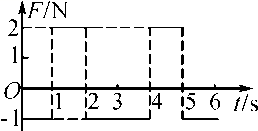
\includegraphics[width=1.17014in,height=0.59444in]{media/image248.png}\end{center}

A.该物体将始终向一个方向运动

B.3 s末该物体回到原出发点

C.0~3 s内,合力F的冲量等于零,功也等于零

D.2~4 s内,合力F的冲量不等于零,功却等于零
\begin{solution}
	图线和横坐标所围的面积等于冲量,0~1秒内的冲量为负,说明速度沿负方向,而1~2秒内冲量为正,且大于0~1秒内的冲量,即速度的方向发生变化,所以选项A错误;0~3秒内,合力F的冲量为零,即物体0秒时的速度和3秒时的速度一样,故0~3秒内合力F的冲量等于零,功也等于零,选项C正确;分析运动过程如图所示,可以得到3秒末物体回到原出发点,选项B正确;2~4秒内,合力F的冲量不等于零,物体2秒时和4秒时速度大小相等,根据动能定理,2~4秒内合力F做的功为零,故选项D正确.
\end{solution}

\begin{center}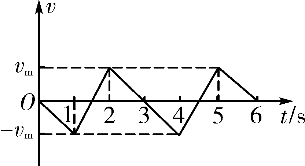
\includegraphics[width=1.38681in,height=0.75486in]{media/image249.png}\end{center}
\newpage
\subsection{动量定理及其应用}

\begin{center}
\includegraphics[width=0.70764in,height=0.12292in]{media/image37.png}

\textbf{动量定理的两个重要应用}
\end{center}

(1)应用$I\neq \Delta p$求变力的冲量

如果物体受到大小或方向改变的力的作用,则不能直接用I=Ft求变力的冲量,可以求出该力作用下物体动量的变化$\Delta p$,等效代换变力的冲量I.

(2)应用$\Delta p$=F$\Delta$t求动量的变化

例如,在曲线运动中,速度方向时刻在变化,求动量变化($\Delta p=p_2-p_1$)需要应用矢量运算方法,计算比较复杂,如果作用力是恒力,可以求恒力的冲量,等效代换动量的变化.

{[}例2{]}(2017·吉林长春质检)有一个质量为0.5 kg的篮球从h=0.8m的高度落到水平地板上,每弹跳一次上升的高度总等于前一次的0.64倍,且每次球与地面接触时间相等,空气阻力不计,与地面碰撞时,篮球重力可忽略.(重力加速度g取$10m/s^2$)

(1)第一次球与地板碰撞,地板对球的冲量为多少?

(2)相邻两次球与地板碰撞的平均冲力大小之比是多少?

\begin{solution}
	(1)3.6 N·s (2)5:4
	
	(1)篮球原高度为h,与地面第一次碰前瞬时速度为$v_{0}=\sqrt{2 g h}=\sqrt{2 \times 10 \times 0.8} \mathrm{m} / \mathrm{s}=4 \mathrm{m} / \mathrm{s}$,由$v^2=2gh$可知碰后的速度为$v_{0}=\sqrt{2 g h}=\sqrt{2 \times 10 \times 0.8} \mathrm{m} / \mathrm{s}=4 \mathrm{m} / \mathrm{s}$.

选向上为正方向,由动量定理有

$I=m v_{1}-\left(-m v_{0}\right)=1.8 m v_{0}=1.8 \times 0.5 \times 4 \mathrm{N} \cdot \mathrm{s}=3.6 \mathrm{N} \cdot \mathrm{s}$.

(2)第二次碰前瞬时速度和第二次碰后瞬时速度关系为$v_{2}=0.8 v_{1}=0.8^{2} v_{0}=0.64 v_{0}$.

设两次碰撞中地板对球的平均冲力分别为F1、F2,选向上为正方向,由动量定理有

$v_{2}=0.8 v_{1}=0.8^{2} v_{0}=0.64 v_{0}$,

$F_{2} t=m v_{2}-\left(-m v_{1}\right)=1.8 m v_{1}=1.44 m v_{0}$,

$F_1$:$F_2$=5:4.

容易知道,任意相邻两次球与地板碰撞的平均冲力大小之比均为5:4.
\end{solution}


{[}例3{]}(2018·湖北黄冈模拟)一股水流以10m/s的速度从喷嘴竖直向上喷出,喷嘴截面积为$0.5 cm^2$,有一质量为0.32kg的球,因受水对其下侧的冲击而停在空中,若水冲击球后速度变为0,则小球停在离喷嘴多高处?(g取$10m/s^2$)
\begin{solution}
	1.8 m
\end{solution}

\begin{center}
\includegraphics[width=0.70764in,height=0.12292in]{media/image25.png}

\textbf{应用动量定理解题的基本思路}
\end{center}


\begin{center}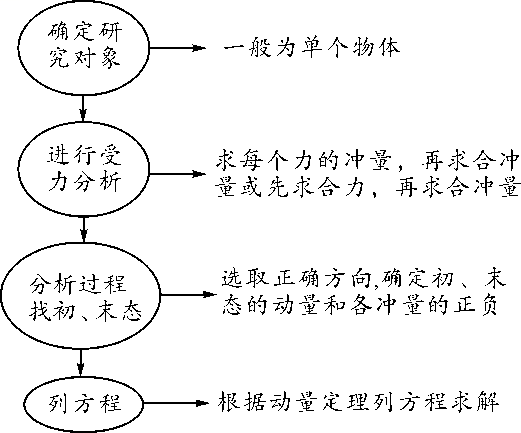
\includegraphics[width=2.36806in,height=1.97153in]{media/image250.png}\end{center}

	

\subsection{动量守恒定律及其应用}

1.动量守恒定律的``五性''

\begin{longtable}[]{@{}ll@{}}
\toprule
条件性 & 首先判断系统是否满足守恒条件(合力为零)\tabularnewline
\midrule
\endhead
相对性 & 公式中$\boldsymbol{v}_{1}, \boldsymbol{v}_{2}, \boldsymbol{v}_{1}^{\prime}, \boldsymbol{v}_{2}^{\prime}$必须相对于同一个惯性系\tabularnewline
同时性 &
公式中$v_1$、$v_2$是在相互作用前同一时刻的速度,$v_1^\prime$、$v_2^\prime$是相互作用后同一时刻的速度\tabularnewline
矢量性 &
应先选取正方向,凡是与选取的正方向一致的动量为正值,相反为负值\tabularnewline
普适性 & 不仅适用于低速宏观系统,也适用于高速微观系统\tabularnewline
\bottomrule
\end{longtable}

2.应用动量守恒定律时的注意事项

(1)动量守恒定律的研究对象都是相互作用的物体组成的系统.系统的动量是否守恒,与选择哪几个物体作为系统和分析哪一段运动过程有直接关系.

(2)分析系统内物体受力时,要弄清哪些力是系统的内力,哪些力是系统外的物体对系统的作用力.

{[}例4{]}(2017·广西南宁模拟)如图所示,质量均为m的小车和木箱紧挨着静止在光滑的水平冰面上,质量为2m的小孩站在小车上用力向右迅速推出木箱,木箱相对于冰面运动的速度为v,木箱运动到右侧墙壁时与竖直墙壁发生弹性碰撞,反弹后能被小孩接住.求:

\begin{center}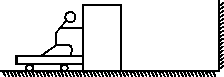
\includegraphics[width=1.01875in,height=0.34931in]{media/image251.png}\end{center}

(1)小孩接住箱子后共同速度的大小;

(2)若小孩接住箱子后再次以相对于冰面的速度v将木箱向右推出,木箱仍与竖直墙壁发生弹性碰撞,判断小孩能否再次接住木箱.
\begin{solution}
	(1)$\dfrac{v}{2}$ (2)见解析
	
	(1)取向左为正方向,木箱与墙发生弹性碰撞,速度反向.根据动量守恒定律,推出木箱的过程中$0=(m+2 m) v_{1}-mv$,接住木箱的过程中$m v+(m+2 m) v_{1}=(m+m+2 m) v_{2}, \quad v_{2}=\dfrac{v}{2}$.

(2)若小孩第二次将木箱推出,设小孩和小车向左的速度为$v_3$,根据动量守恒定律$4 m v_{2}=3 m v_{3}-m v, v_{3}=v$,故无法再次接住木箱.
\end{solution}


\begin{center}
\includegraphics[width=0.70764in,height=0.12292in]{media/image25.png}

\textbf{动量守恒定律解题的基本步骤}
\end{center}


(1)明确研究对象,确定系统的组成;(系统包括哪几个物体及研究的过程)

(2)进行受力分析,判断系统动量是否守恒;(或某一方向上动量是否守恒)

(3)规定正方向,确定初、末状态动量;

(4)由动量守恒定律列出方程;

(5)代入数据,求出结果,必要时讨论说明.
\newpage
\subsection{碰撞问题}

碰撞遵守的规律

(1)动量守恒,即$p_{1}+p_{2}=p_{1}^{\prime}+p_{2}^{\prime}$.

(2)动能不增加,即$E_{\mathrm{k} 1}+E_{\mathrm{k} 2} \geq E_{\mathrm{k} 1}^{\prime}+E_{\mathrm{k} 2}^{\prime}$ 或 $\dfrac{p_{1}^{2}}{2 m_{1}}+\dfrac{p_{2}^{2}}{2 m_{2}} \geq \dfrac{p^{\prime 2}}{2 m_{1}}+\dfrac{p^{\prime 2}}{2 m_{2}}$. 

(3)速度要合理

\ding{172}碰前两物体同向,则$v_{\text{后}}>v_{\text{前}}$;碰后,原来在前的物体速度一定增大,且$v_{\text{前}}^\prime>v_{\text{后}}^\prime$.

\ding{173}两物体相向运动,碰后两物体的运动方向不可能都不改变.

{[}例5{]}如图,在足够长的光滑水平面上,物体A、B、C位于同一直线上,A位于B、C之间.A的质量为m,B、C的质量都为M,三者均处于静止状态.现使A以某一速度向右运动,求m和M之间应满足什么条件,才能使A只与B、C各发生一次碰撞.设物体间的碰撞都是弹性碰撞.

\begin{center}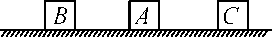
\includegraphics[width=1.23611in,height=0.17014in]{media/image252.png}\end{center}
\begin{solution}$(\sqrt{5}-2) M \leq m<M$

	设A运动的初速度为v0,A向右运动与C发生碰撞,由动量守恒定律得$m v_{0}=m v_{1}+M v_{2}$,

由机械能守恒得$\dfrac{1}{2} m v_{0}^{2}=\dfrac{1}{2} m v_{1}^{2}+\dfrac{1}{2} M v_{2}^{2}$,

可得$v_{1}=\dfrac{m-M}{m+M} v_{0}, \quad v_{2}=\dfrac{2 m}{m+M} v_{0}$.

要使得A与B能发生碰撞,需要满足$v_{1}<0, \quad$ 即 $m<M$,

A反向向左运动与B发生碰撞过程,有$m v_{1}=m v_{3}+M v_{4}$,

$\dfrac{1}{2} m v_{1}^{2}=\dfrac{1}{2} m v_{3}^{2}+\dfrac{1}{2} M v_{4}^{2}$,

整理可得$v_{3}=\dfrac{m-M}{m+M} v_{1}=\left(\dfrac{m-M}{m+M}\right)^{2} v_{0}, \quad v_{4}=\dfrac{2 m}{m+M} v_{1}$.

由于m<M,所以A还会向右运动,根据要求不发生第二次碰撞,需要满足$v3\leq v2$,

即$\dfrac{2 m}{m+M}_{00 \geq}\left(\dfrac{m-M}{m+M}\right)^{2} v_{0}$,

整理可得$m^{2}+4 M m \geq M^{2}$,

解方程可得$m \geq(\sqrt{5}-2) M$,

所以使A只与B、C各发生一次碰撞,需满足

$(\sqrt{5}-2) M \leq m<M$.
\end{solution}


\begin{center}
\includegraphics[width=0.70764in,height=0.12292in]{media/image13.png}

\textbf{碰撞问题解题策略}
\end{center}


(1)抓住碰撞的特点和不同种类碰撞满足的条件,列出相应方程求解.

(2)可熟记一些公式,例如``一动一静''模型中,两物体发生弹性正碰后的速度满足$v_{1}=\dfrac{m_{1}-m_{2}}{m_{1}+m_{2}} v_{0}, \quad v_{2}=\dfrac{2 m_{1}}{m_{1}+m_{2}} v_{0}$.

(3)熟记弹性正碰的一些结论,例如,当两球质量相等时,两球碰撞后交换速度;当$m_{1} \gg m_{2},$ 日 $v_{20}=0$时,碰后质量大的速率不变,质量小的速率为$2 v_{0} ; \quad$ 当 $m_{1} \ll m_{2}, \quad$ 目 $v_{20}=0$时,碰后质量小的球原速率反弹.
\newpage
\subsection{爆炸、反冲和``人船模型''}

1.爆炸的特点

(1)动量守恒:由于爆炸是在板短的时间内完成的,发生爆炸时物体间的相互作用力远远大于受到的外力,所以在爆炸过程中,系统的总动量守恒.

(2)动能增加:在爆炸过程中,由于有其他形式的能量(如化学能)转化为动能,所以爆炸前后系统的总动能增加.

(3)位置不变:爆炸的时间极短,因而在作用过程中,物体产生的位移很小,一般可忽略不计,可以认为爆炸后仍然从爆炸前的位置以新的动量开始运动.

{[}例6{]}(2018·河南六市一联)如图所示,光滑水平面上有三个滑块A、B、C,质量关系是$m_{A}=m_{C}=m, m_{B}=\dfrac{m}{2}$.开始时滑块B、C紧贴在一起,中间夹有少量炸药,处于静止状态,滑块A以速度$v_0$正对B向右运动,在A未与B碰撞之前,引爆了B、C间的炸药,炸药爆炸后B与A迎面碰撞,最终A与B黏在一起,以速率$v_0$向左运动.求:

(1)炸药爆炸过程中炸药对C的冲量;

(2)炸药的化学能有多少转化为机械能?

\begin{center}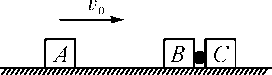
\includegraphics[width=1.23611in,height=0.33958in]{media/image253.png}\end{center}

\begin{solution}
	(1)$\dfrac{5}{2} m v_{0}$,水平向右 (2)$\dfrac{75}{8} m v_{0}^{2}$
\end{solution}
2.反冲

(1)现象:物体的不同部分在内力的作用下向相反方向运动的现象.

(2)特点:一般情况下,物体间的相互作用力(内力)较大,因此系统动量可能是动量守恒、动量近似守恒或某一方向上动量守恒.反冲运动中机械能往往不守恒.

(3)实例:喷气式飞机、火箭等都是利用反冲运动的实例.

{[}例7{]}一质量为M的航天器,正以速度$v_0$在太空中飞行,某一时刻航天器接到加速的指令后,发动机瞬间向后喷出一定质量的气体,气体喷出时速度大小为$v_1$,加速后航天器的速度大小为$v_2$,则喷出气体的质量m为( C )

A.$m=\dfrac{v_{2}-v_{0}}{v_{1}} M$   

B.$m=\dfrac{v_{2}}{v_{2}+v_{1}} M$

C.$\dfrac{v_{2}-v_{0}}{v_{2}+v_{1}} M$   

D.$\dfrac{v_{2}-v_{0}}{v_{2}-v_{1}} M$

3.``人船模型''

若系统在全过程中动量守恒,则这一系统在全过程中平均动量也守恒.如果系统由两个物体组成,且相互作用前均静止,相互作用中均发生运动,则由$m_{1} \overline{v_{1}}-m_{2} \overline{v_{2}}=0$,得$m_{1} x_{1}=m_{2} x_{2}$. 



\begin{center}
\includegraphics[width=0.70764in,height=0.12292in]{media/image13.png}

\textbf{利用``人船模型''解题需注意两点}
\end{center}


(1)条件

\ding{172}系统的总动量守恒或某一方向上的动量守恒.

\ding{173}构成系统的两物体原来静止,因相互作用而反向运动.

\ding{174}$x_1$、$x_2$均为沿动量方向相对于同一参考系的位移.

(2)解题关键是画出初、末位置,确定各物体位移关系.

\begin{problemset}
	\item 基础概念
	\begin{itemize}
		\item 质点系:包含两个或两个以上互相有联系的的质点组成的力学系统叫做质点系(或质点组)。
		\item 质心:质量中心简称质心,指物质系统上被认为质量集中于此的一个假想点。
		\item 质心系:质心坐标系是将直角坐标系的坐标原点始终选取在质点组的质心上,坐标轴的方向始终与某个固定参考系(惯性系)的坐标轴保持平行的平动坐标系。对于不受外力作用的质点组(孤立体系)或所受外力的矢量和为零的质点组,其质心系是惯性系.对于受外力作用的质点组,其质心系是非惯性系。
		\item 动量中心系:动量中心系(Center-of-momentumframe)是人为选取的一个惯性系,在此参考系中,系统的总动量为零。动量中心系又叫做零动量系(zero-momentumframe)。
		
		动量中心系的特例是质心参考系,即原点固定在体系质心的动量中心系。
	\end{itemize}
	\item 柯尼希定理,资用能
	\begin{itemize}
		\item 柯尼希定理:质点系在某参考系中的动能等于质心系中的动能与质点系随质心整体平动的质心动能之和。
		\item 高中两体碰撞问题的简化模型
		
		设两质点质量为$m_1,m_2$,速度为$v_1,v_2$,则质心速度
		\begin{equation}
			v_c=\dfrac{m_{1} v_{1}+m_{2} v_{2}}{m_{1}+m_{2}}
		\end{equation}
		$m_1$相对于质心的速度为
		\begin{equation}
			v_{1c}=v_1-v_c=v_1-\dfrac{m_{1} v_{1}+m_{2} v_{2}}{m_{1}+m_{2}}=\dfrac{m_2(v_1-v_2)}{m_1+m_2}
		\end{equation}
		$m_2$相对于质心的速度为
		\begin{equation}
			v_{2c}=v_2-v_c=v_2-\dfrac{m_{1} v_{1}+m_{2} v_{2}}{m_{1}+m_{2}}=\dfrac{m_1(v_2-v_1)}{m_1+m_2}
		\end{equation}
		由柯尼希定理得
		\begin{equation}
			E_k=\dfrac{1}{2}Mv_c^2+\dfrac{1}{2}m_1v_{1c}^2+\dfrac{1}{2}m_2v_{2c}^2=\dfrac{1}{2}(m_1+m_2)v_c^2+\dfrac{1}{2}\dfrac{m_1m_2}{m_1+m_2}(v_1-v_2)^2
		\end{equation}
		公式(6.4)的动能由质心系中的动能(6.5)以及质点系随质心整体平动的质心动能(6.6)两部分组成
		\begin{equation}
			E_k=\dfrac{1}{2}(m_1+m_2)v_c^2
		\end{equation}
		
		\begin{equation}
			E_k=\dfrac{1}{2}\dfrac{m_1m_2}{m_1+m_2}(v_1-v_2)^2
		\end{equation}
		\item 结论
		
		公式(6.6)可以与能量守恒等效,在完全弹性碰撞的计算中,能量守恒公式可以直接用资用能守恒代替,在化简后会变成相对速度守恒:$\lvert v_1-v_2 \rvert=\lvert v_1^\prime-v_2^\prime \rvert$,去掉绝对值后:$v_1-v_2=v_2^\prime-v_1^\prime $;非完全弹性碰撞中,损失的能量为初末状态资用能差值。
	\end{itemize}
	\newpage
	\item 速度增量
	
	上面我们使用柯尼希定理中的资用能表达式优化了碰撞的计算,接下来我们继续优化完全弹性碰撞的计算。
	
	设两质点质量为$m_1,m_2$,速度为$v_1,v_2$,完全非弹性碰撞速度为$v_c$,完全弹性碰撞速度为$v_1^\prime$,$v_2^\prime$。对任一物体分析:初速度到共同速度的增量等于共同速度到末速度的增量。即:
		\begin{equation}
			v_c-v_1=v_1^\prime-v_c
		\end{equation}
		\begin{equation}
			v_c-v_2=v_2^\prime-v_c
		\end{equation}
	至此,我们已经可以口算完全弹性碰撞了。

	下面给出速度增量的几何证明:
	\begin{center}
		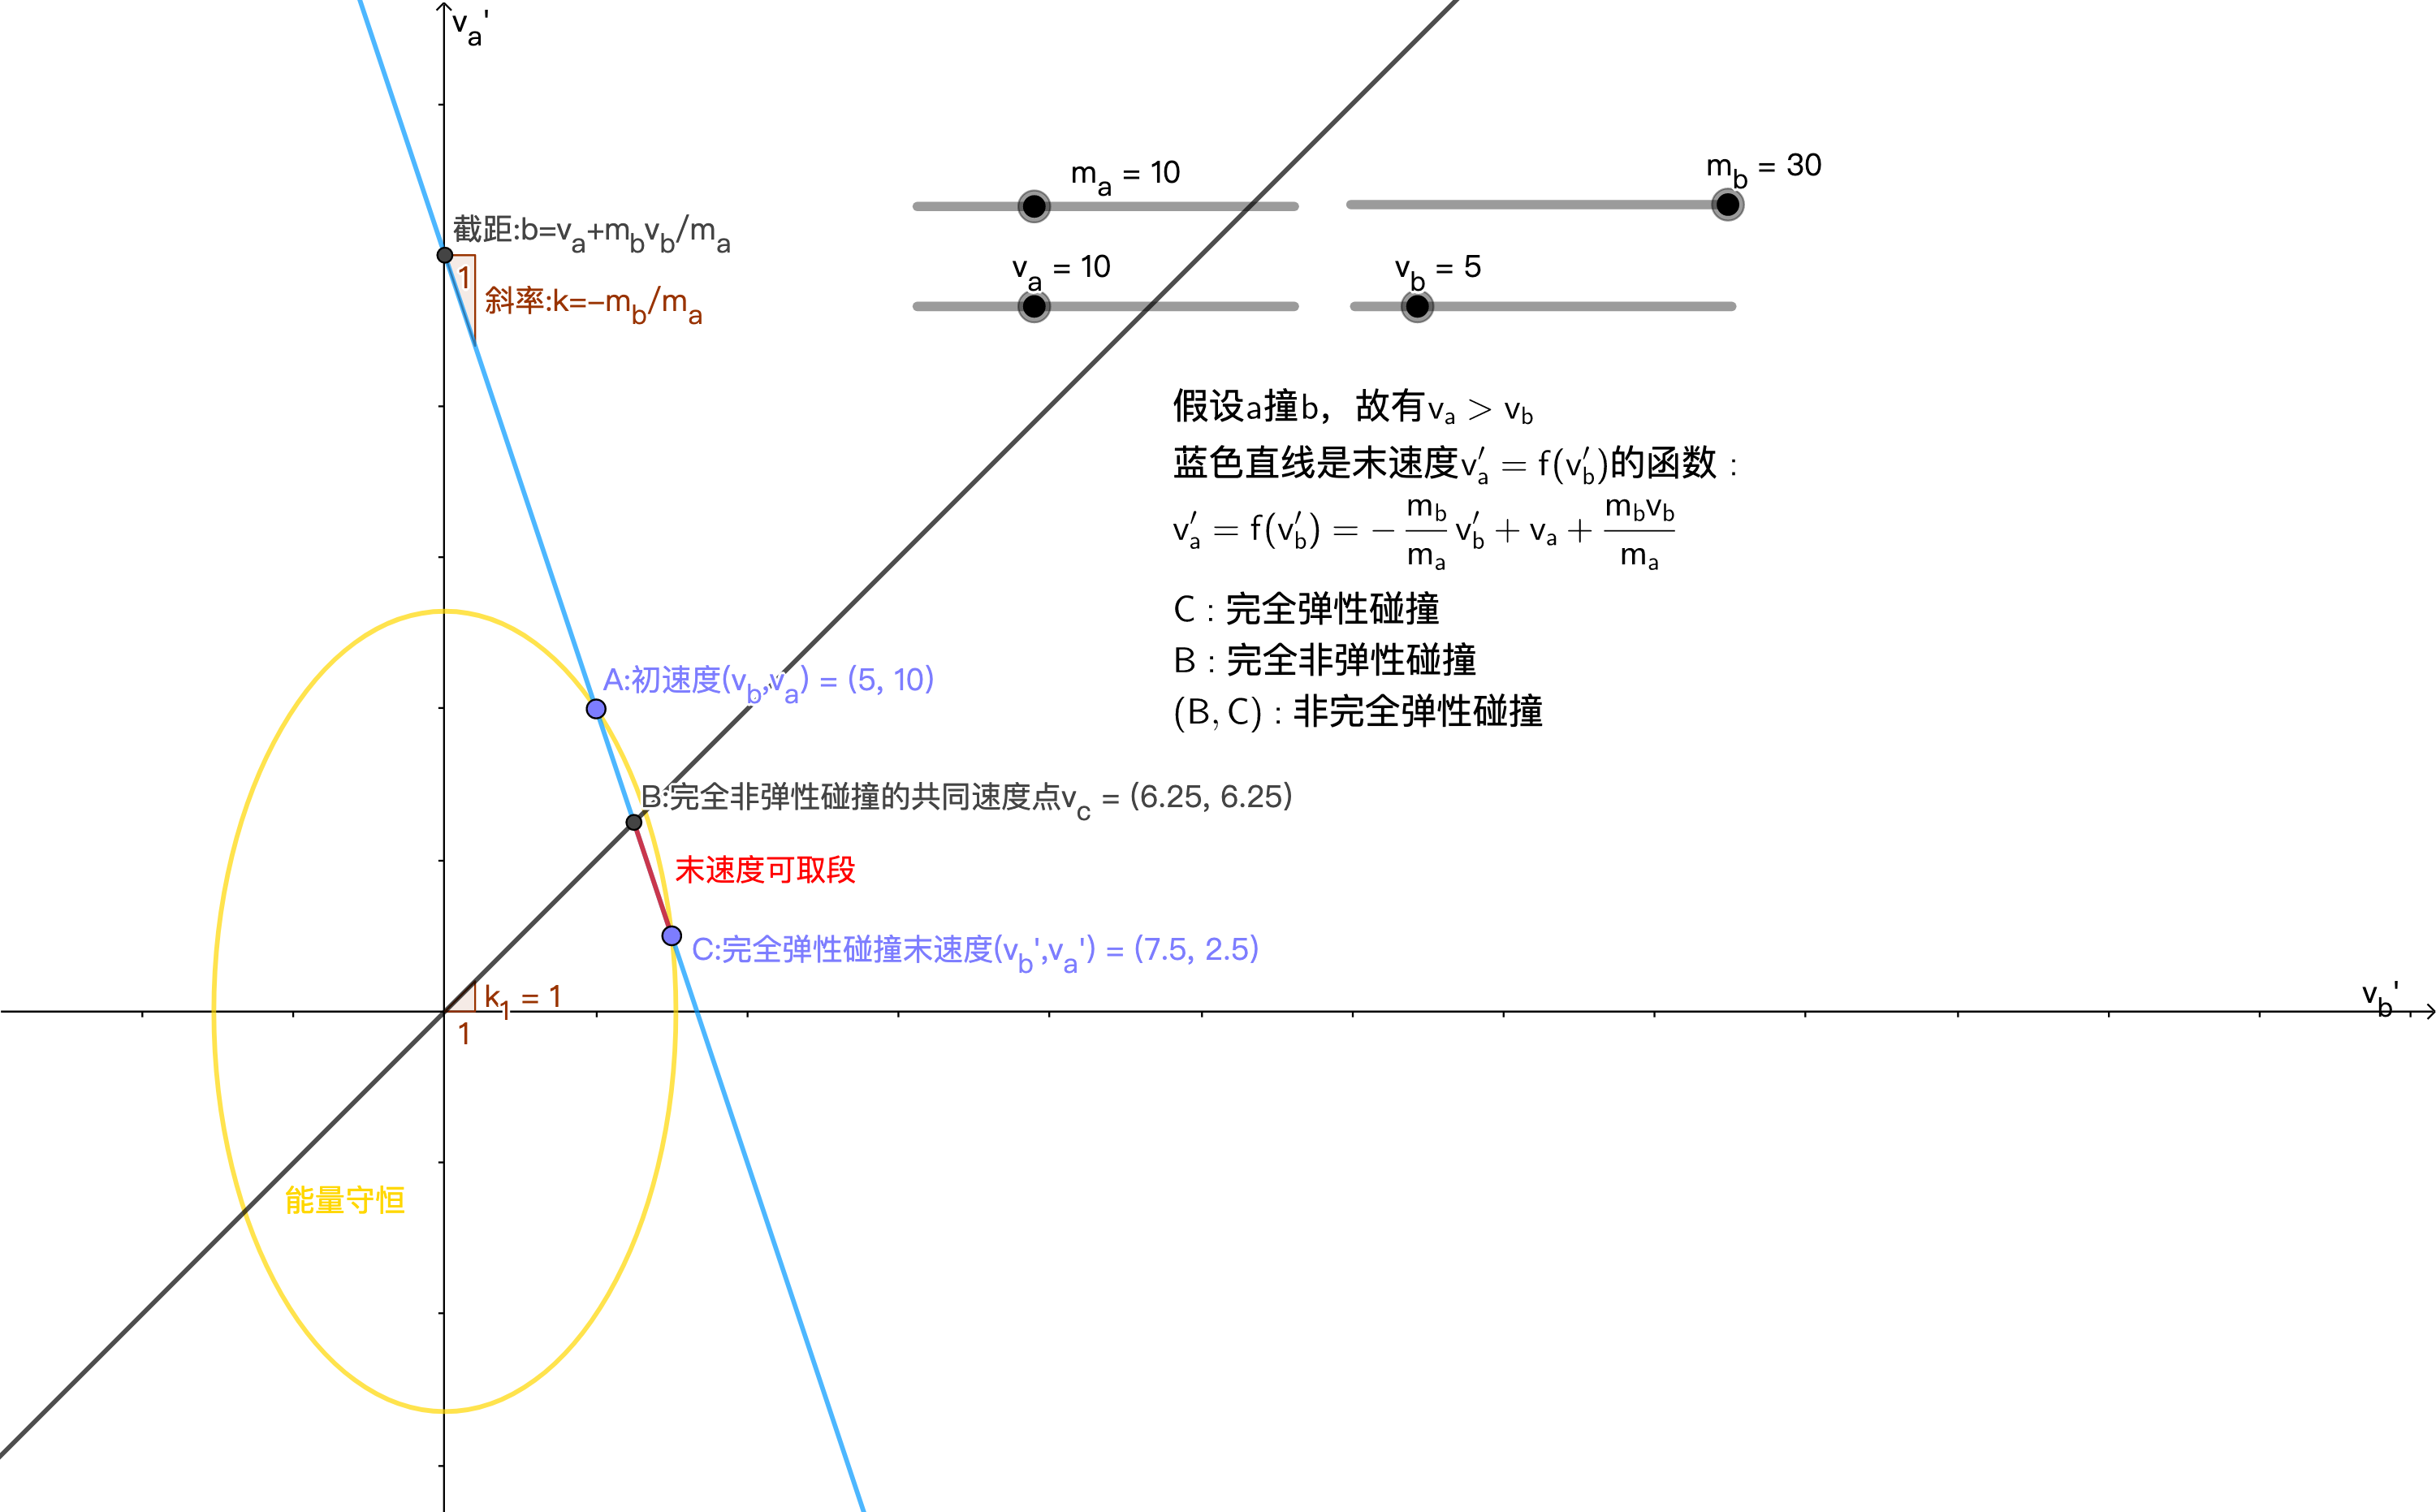
\includegraphics[width=13cm]{media/61.png}
	\end{center}
	图片来源:\href{https://www.geogebra.org/classic/dma875ya}{https://www.geogebra.org/classic/dma875ya}
	
	如图,坐标系横轴为b的末速度,纵轴为a的末速度。蓝色函数是动量守恒,点A是a,b的初速度,由于初速度$v_a>v_b$,碰撞后有$v_a<=v_b$,所以过坐标系原点作函数y=x,函数上及右边的区域符合$v_a<=v_b$。函数y=x交函数动量定理于点B,则B点是共速点。由柯尼希定理可知相对速度不会增加,作点A关于点B的对称点C,则集合[B,C]上的点满足动量守恒及柯尼希定理。

	由于相对速度证明和能量守恒证明可以替换,能量守恒方程(黄色)也可证明BC段的有效性。
	\newpage
	\item 动量与$\pi$
	
	美国东伊利诺大学Gregory Galperin教授在1995年东伊利诺斯大学数学讨论会上首次报告了两球与墙壁三者间的总碰撞次数与圆周率之间的关系,当他在报告中公布这个结论时,听众们开始都觉得难以置信,但在给出证明后,听众们又纷纷表示信服。2003年,Gregory Galperin教授在论文\href{https://github.com/Campanulata/LectureNotesOnHighSchoolPhysics/blob/master/data/PLAYING%20POOL%20WITH%20%CF%80.pdf}{《Playing pool with $\pi$ — The number $\pi$ from a billiard point of view》}中公布了证明过程,他的主要证明思路是将碰撞次数问题转化为类似于光学中平面镜反射次数问题。
	知名up主Grant Sanderson(3B1B)也在视频网站上分享了利用光学的证明:\href{https://www.bilibili.com/video/BV1Mb41187jL}{https://www.bilibili.com/video/BV1Mb41187jL}

	下面给出几何证明
	\begin{center}
		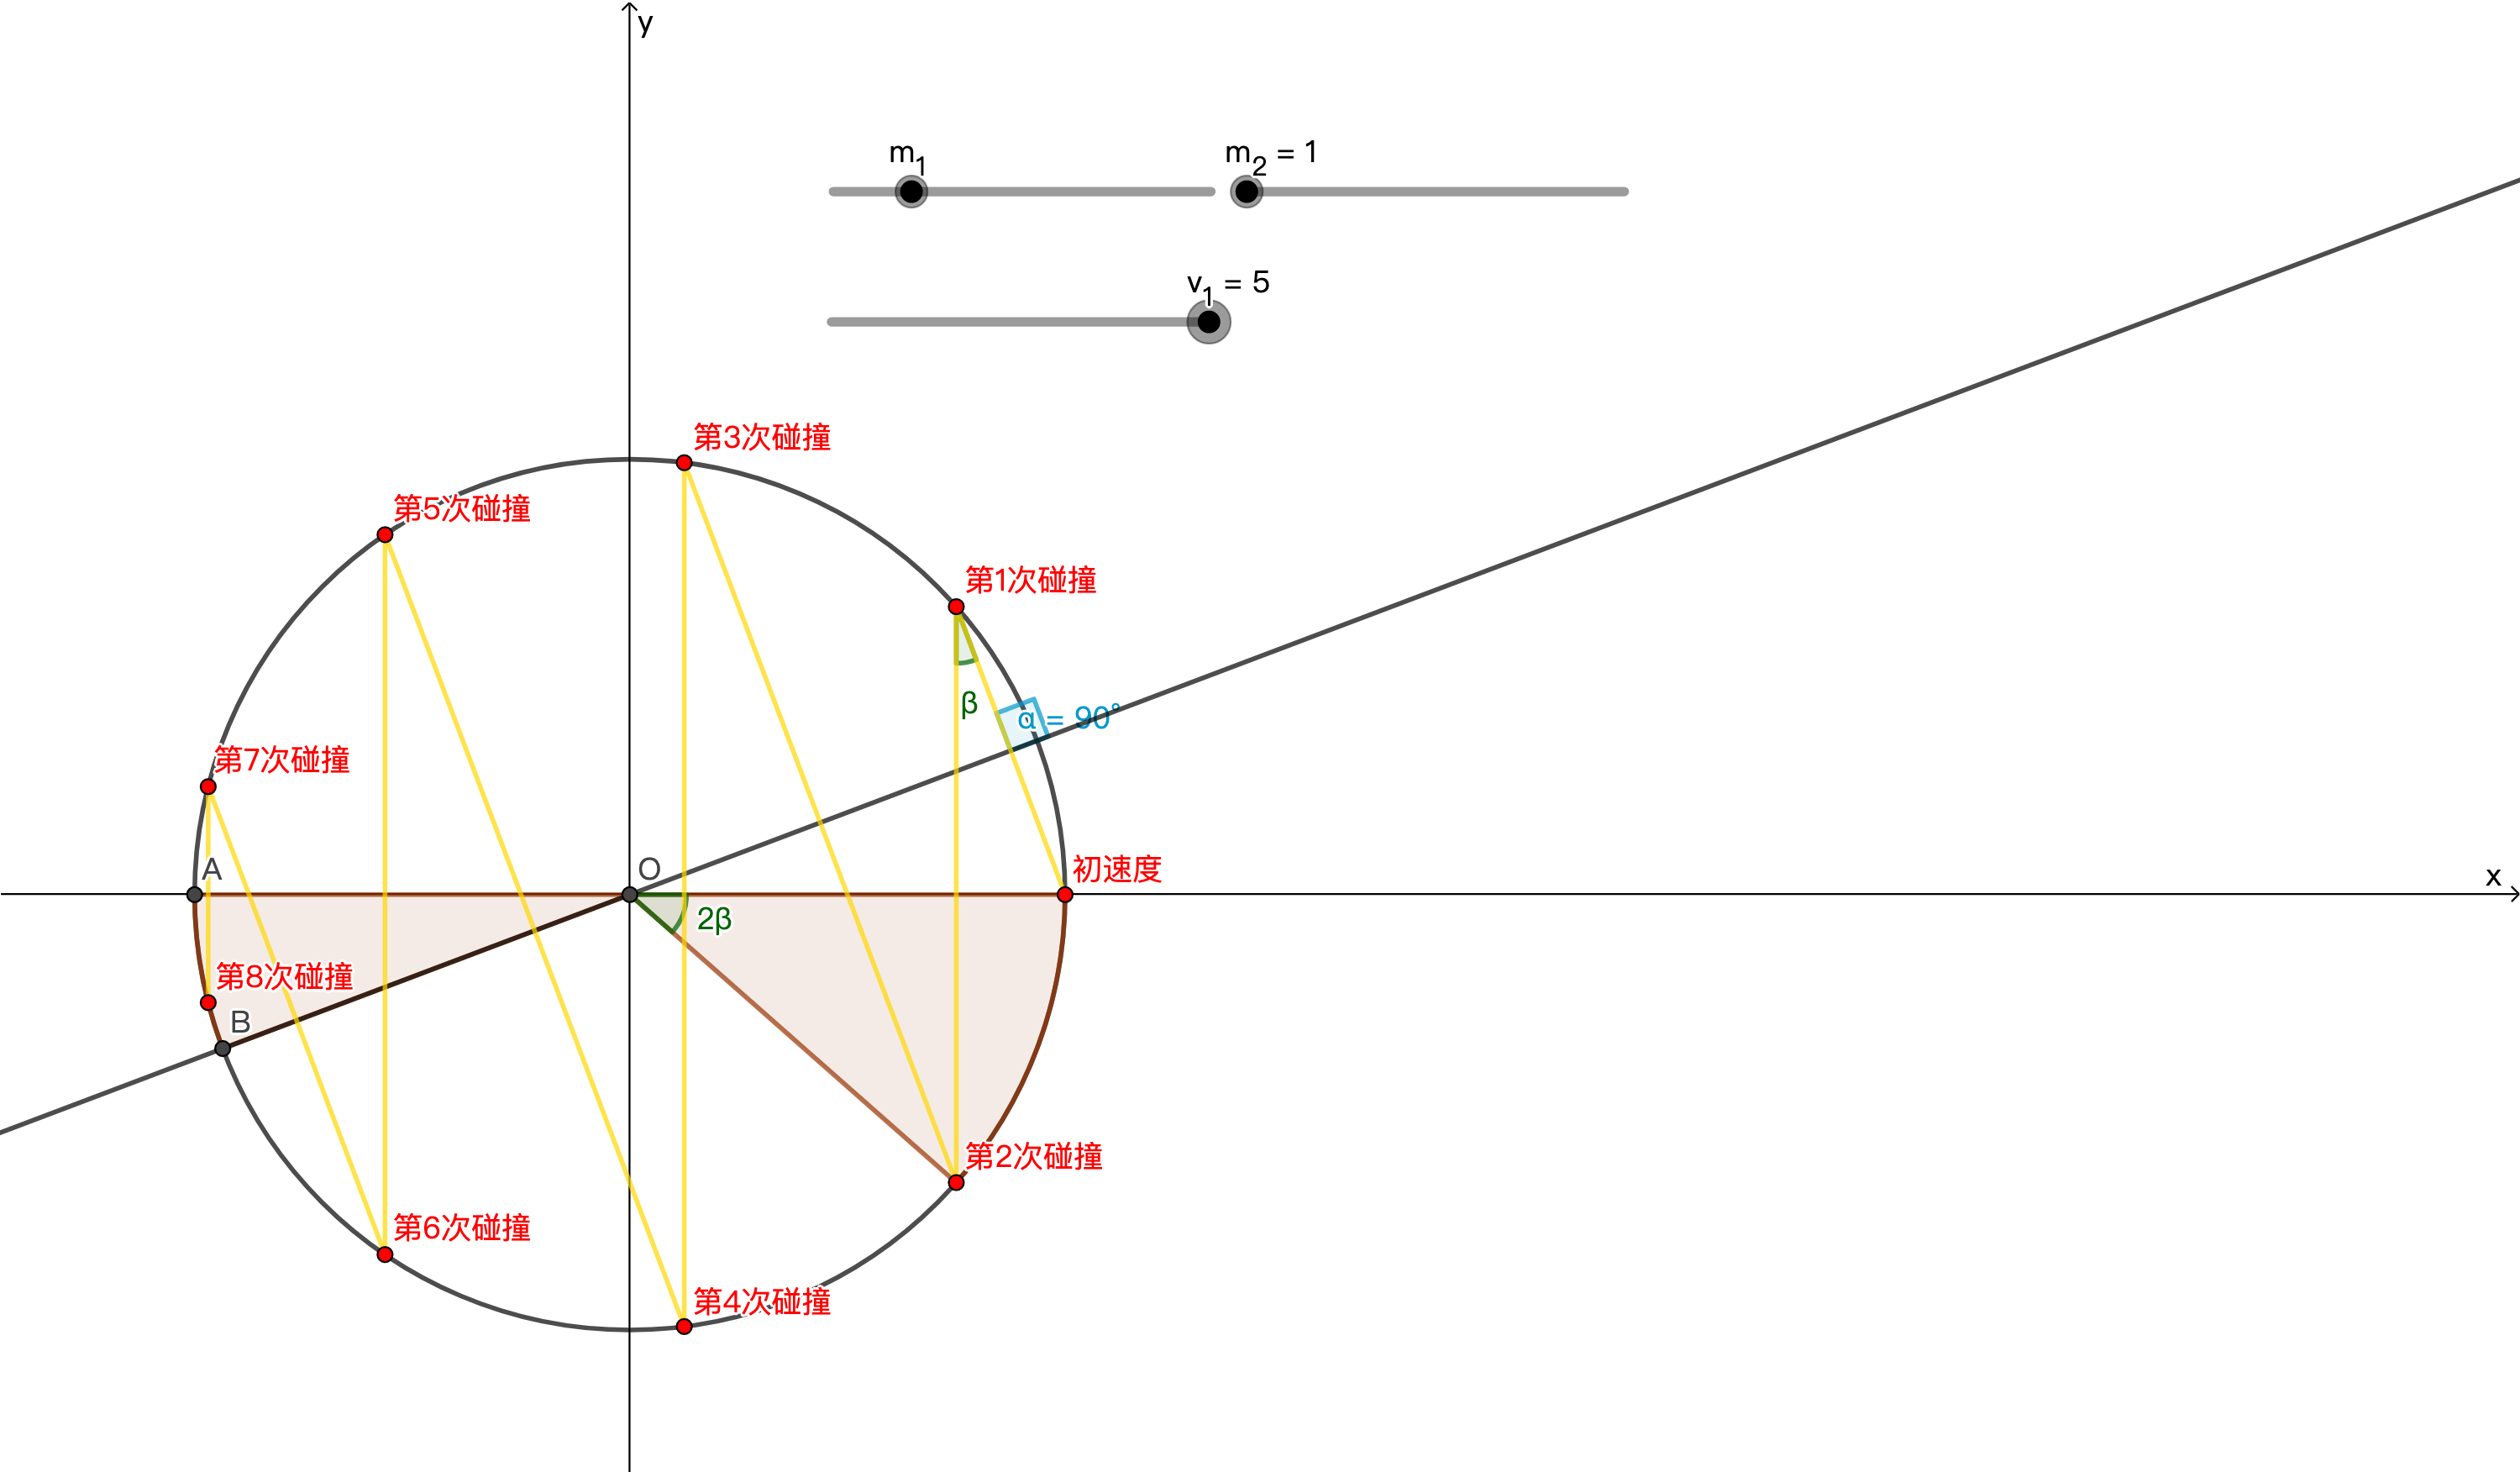
\includegraphics[width=13cm]{media/62.png}
	\end{center}
	图片来源:\href{https://www.geogebra.org/classic/xmq7m6dt}{https://www.geogebra.org/classic/xmq7m6dt}
	假设可视为质点的物体A质量为$m_1$,以初速度为$v_0$撞击质量为$m_2$的物体B。B的前方有一堵墙。物体与物体,物体与墙面的碰撞均为完全弹性碰撞。若以$v_1,v_2$分别表示A,B任意时刻的速度,规定初速度方向为正方向,则:
	\begin{equation}
		m_1v_1+m_2v_2=m_1v_0
	\end{equation}
	\begin{equation}
		\frac{1}{2}m_1v_1^2+\frac{1}{2}m_2v_2^2=\frac{1}{2}m_1v_0^2
	\end{equation}
	令$x=\sqrt{m_1}v_1$,$y=\sqrt{m_2}v_2$则:
	\begin{equation}
		\sqrt{m_1}x+\sqrt{m_2}y=m_1v_0
	\end{equation}
	\begin{equation}
		\frac{1}{2}x^2+\frac{1}{2}y^2=\frac{1}{2}m_1v_0^2
	\end{equation}
	如图作出方程(6.11)(6.12),图中已将(6.11)隐藏,应该是与线段[初速度,第1次碰撞]共线的直线。与圆交于两点,分别是碰撞前的初速度和第1次碰撞后的速度。随后B与墙面发生碰撞,速度反向,作关于x轴对称点,得到B与墙面碰撞后的速度。由于动量守恒,过点(第2次碰撞)作动量守恒的平行线得到第3次碰撞。同理,可得到第n次碰撞的点。
	\newpage
	接下来我们将在图中表示碰撞中止:
	模型中碰撞中止的条件是:$v_1,v_2$均与初速度$v_0$反向\ding{172},且$\vert v_1\vert >\vert v_2\vert$\ding{173},则:
	\begin{align*}
		v_1&<v_2\\
		\dfrac{x}{\sqrt{m_1}}&<\dfrac{y}{\sqrt{m_2}}\\
		y&>\sqrt{\frac{m_2}{m_1}}x
	\end{align*}
	在图中作出$y=\sqrt{\frac{m_2}{m_1}}x$的图像,由于斜率与动量守恒斜率互成负倒数,所以互相垂直。

	满足条件\ding{172}的区域为第三象限,满足条件\ding{173}的区域为$y>\sqrt{\frac{m_2}{m_1}}x$的左边。所以碰撞后的速度在$\overset{\frown}{AB}$上,碰撞中止。

	图示为第8次碰撞后中止。以初速度与第2次碰撞间的弧为例,设圆周角为$\beta$,则其圆心角为$2\beta$,观察可知每发生一次碰撞,圆周就会被分割出一个圆心角为$2\beta$的弧。设该过程发生的碰撞次数为n,则:
	\begin{equation}
		n\times 2\beta<2\pi
	\end{equation}
	当$\frac{m_1}{m_2}=100^k(k=1,2,3\cdots)$时,
	\begin{align*}
		\frac{m_1}{m_2}&\ge 100\\
		\frac{m_2}{m_1}&\le \frac{1}{100}\\
		\sqrt{\frac{m_2}{m_1}}&\le 0.1\\
		\tan\beta&\le 0.1
	\end{align*}
	由于$\tan\beta\rightarrow 0$
	\begin{equation}
		\tan\beta\approx\beta
	\end{equation}
	联立公式(6.13)(6.14)
	\begin{align*}
		n\times 2\tan\beta&<2\pi\\
		n\times \sqrt{\frac{m_2}{m_1}}&<\pi\\
		n&<\sqrt{\frac{m_1}{m_2}}\pi
	\end{align*}
	由于n为正整数,所以当k取1,2,3$\cdots$时,n为31,314,3141$\cdots$
\end{problemset}
